% Options for packages loaded elsewhere
\PassOptionsToPackage{unicode}{hyperref}
\PassOptionsToPackage{hyphens}{url}
%
\documentclass[
  12pt,
]{article}
\usepackage{amsmath,amssymb}
\usepackage{iftex}
\ifPDFTeX
  \usepackage[T1]{fontenc}
  \usepackage[utf8]{inputenc}
  \usepackage{textcomp} % provide euro and other symbols
\else % if luatex or xetex
  \usepackage{unicode-math} % this also loads fontspec
  \defaultfontfeatures{Scale=MatchLowercase}
  \defaultfontfeatures[\rmfamily]{Ligatures=TeX,Scale=1}
\fi
\usepackage{lmodern}
\ifPDFTeX\else
  % xetex/luatex font selection
\fi
% Use upquote if available, for straight quotes in verbatim environments
\IfFileExists{upquote.sty}{\usepackage{upquote}}{}
\IfFileExists{microtype.sty}{% use microtype if available
  \usepackage[]{microtype}
  \UseMicrotypeSet[protrusion]{basicmath} % disable protrusion for tt fonts
}{}
\makeatletter
\@ifundefined{KOMAClassName}{% if non-KOMA class
  \IfFileExists{parskip.sty}{%
    \usepackage{parskip}
  }{% else
    \setlength{\parindent}{0pt}
    \setlength{\parskip}{6pt plus 2pt minus 1pt}}
}{% if KOMA class
  \KOMAoptions{parskip=half}}
\makeatother
\usepackage{xcolor}
\usepackage[margin=1in]{geometry}
\usepackage{longtable,booktabs,array}
\usepackage{calc} % for calculating minipage widths
% Correct order of tables after \paragraph or \subparagraph
\usepackage{etoolbox}
\makeatletter
\patchcmd\longtable{\par}{\if@noskipsec\mbox{}\fi\par}{}{}
\makeatother
% Allow footnotes in longtable head/foot
\IfFileExists{footnotehyper.sty}{\usepackage{footnotehyper}}{\usepackage{footnote}}
\makesavenoteenv{longtable}
\usepackage{graphicx}
\makeatletter
\def\maxwidth{\ifdim\Gin@nat@width>\linewidth\linewidth\else\Gin@nat@width\fi}
\def\maxheight{\ifdim\Gin@nat@height>\textheight\textheight\else\Gin@nat@height\fi}
\makeatother
% Scale images if necessary, so that they will not overflow the page
% margins by default, and it is still possible to overwrite the defaults
% using explicit options in \includegraphics[width, height, ...]{}
\setkeys{Gin}{width=\maxwidth,height=\maxheight,keepaspectratio}
% Set default figure placement to htbp
\makeatletter
\def\fps@figure{htbp}
\makeatother
\setlength{\emergencystretch}{3em} % prevent overfull lines
\providecommand{\tightlist}{%
  \setlength{\itemsep}{0pt}\setlength{\parskip}{0pt}}
\setcounter{secnumdepth}{-\maxdimen} % remove section numbering
\usepackage{titling}
\pretitle{\begin{center}\Huge\bfseries}
\posttitle{\par\end{center}}
\predate{\begin{center}\large}
\postdate{\par\end{center}}
\preauthor{\begin{center}\large}
\postauthor{\par\end{center}}
\usepackage{amsmath}
\usepackage{amsthm}
\usepackage{rotating}
\usepackage{setspace}
\doublespacing
\usepackage{booktabs}
\usepackage{longtable}
\usepackage{array}
\usepackage{multirow}
\usepackage{wrapfig}
\usepackage{float}
\usepackage{colortbl}
\usepackage{pdflscape}
\usepackage{tabu}
\usepackage{threeparttable}
\usepackage{threeparttablex}
\usepackage[normalem]{ulem}
\usepackage{makecell}
\usepackage{xcolor}
\ifLuaTeX
  \usepackage{selnolig}  % disable illegal ligatures
\fi
\usepackage{bookmark}
\IfFileExists{xurl.sty}{\usepackage{xurl}}{} % add URL line breaks if available
\urlstyle{same}
\hypersetup{
  pdftitle={Evaluating the Effect of the RapidRide Program on Bus Reliability in Seattle, WA, Using Bayesian Additive Regression Trees},
  pdfauthor={Peter Silverstein},
  hidelinks,
  pdfcreator={LaTeX via pandoc}}

\title{Evaluating the Effect of the RapidRide Program on Bus Reliability
in Seattle, WA, Using Bayesian Additive Regression Trees}
\author{Peter Silverstein}
\date{2025-04-24}

\begin{document}
\maketitle

\begin{center}
    {\large Draft 1}\\[0.5cm]
    {\large QMSS Master's Thesis}\\[0.5cm]
    {\large Advisor: Dr. Edwin Grimsley}\\[0.5cm]
    {\large Instructor: Dr. Kenneth Grossberger}\\[0.5cm]
\end{center}

\newpage

\tableofcontents

\newpage

\section{Abstract}\label{abstract}

Mass transit systems are a crucial piece in the fabric of any urban
environment. They allow people who don't own cars to access the far
reaches of the city and provide a more sustainable alternative to single
occupancy vehicle traffic. In large part, the success of a transit
system is dependent on its ability to get people where they want to go
and do so with reliability. The present research examines a transit
intervention, the RapidRide bus route upgrade program in Seattle,
Washington, and seeks to determine whether it has a positive effect on
bus reliability. Linear Regression models and a Bayesian Additive
Regression Trees model are applied in a causal inference setting to
estimate the average treatment effect of the RapidRide treatment on the
bus routes that have been upgraded. All models find that the RapidRide
treatment improves reliability. Estimates for this treatment effect
range from a 25 second to nearly 90 second improvement as a result of
the treatment. Because reliability is an attribute that is highly valued
by mass transit riders and because better reliability is associated with
a greater ability to make transfers and travel efficiently, these models
point to the RapidRide upgrade program being a success.

\newpage

\section{1. Introduction}\label{introduction}

Public transit systems play a crucial role in shaping urban environments
by providing residents with affordable, sustainable, and efficient
mobility options. A key factor determining the effectiveness of transit
systems is accessibility---the ease with which riders can reach desired
destinations within a city. Accessibility is often operationalized
through the concept of the Space-Time Prism (STP), which measures the
range of feasible destinations that individuals can reach given
constraints such as travel speed, wait times, and transfers. Within this
framework, transit reliability---the consistency and predictability of
service schedules---is critically important. Unreliable service,
characterized by late or early arrivals, negatively impacts riders'
ability to successfully transfer between routes, thereby reducing
overall accessibility. To address reliability issues without incurring
the substantial costs and timelines associated with major infrastructure
projects like subway or light rail systems, many cities have turned to
Bus Rapid Transit (BRT). BRT encompasses operational strategies such as
bus-only lanes, off-board fare collection, traffic signal priority, and
active headway management to enhance bus service speed and reliability.
Seattle's RapidRide program exemplifies a ``BRT-lite'' approach,
implementing selected BRT features on high-demand bus routes to improve
service quality at relatively lower costs. Despite ongoing investments
in RapidRide upgrades across Seattle's transit network, empirical
evidence regarding their effectiveness remains limited. This paper seeks
to fill this gap by evaluating whether routes upgraded under the
RapidRide program exhibit improved reliability compared to comparable
routes without such upgrades. Using observational data collected from
King County Metro's real-time bus arrival system and employing advanced
causal inference methods---specifically Bayesian Additive Regression
Trees (BART) within a hierarchical modeling framework---this study
estimates the causal impact of RapidRide treatments on transit
reliability. By rigorously accounting for multilevel data structures and
potential confounding variables such as traffic conditions and ridership
demand, the analysis aims to provide robust insights into the
effectiveness of targeted transit interventions in enhancing urban
accessibility through improved schedule adherence.

\section{2. Literature Review}\label{literature-review}

\subsection{2.1 Accessibility and Transit
Reliability}\label{accessibility-and-transit-reliability}

Cities may be understood as complex spatial relationships between
people, places, and services. To a large degree, where an individual is
within a city may determine their ability to access various other
people, places, and services within that city. The related concepts of
access and accessibility (originally formulated by Hansen, 1959) are
central to the field of urban planning and represent the extent to which
any given thing is available to an individual that exists at a given
location. Though access is a broad term that may be operationalized in
various ways, depending on the exact purpose of the research, the
central ideal within designing an urban environment with access in mind
is to give people the maximum ability to get to the places and things
that they want or need to get to (Levinson and Wu, 2020). This may be
done in different ways---land use planning would seek to place relevant
zones (e.g., retail, industrial, residential, etc.) in useful places,
and it may be a further goal of an urban planner to ensure equity in
access between individuals of different social backgrounds (Hansen,
1959). In addition to putting people and things in optimal places, it is
necessary for transportation planners to consider how to design systems
that get people where they need to go in an efficient manner. Within the
framework of urban transportation, mass transit systems provide key
benefits that make them important and relevant subjects of study and
evaluation. Mass transit systems allow people to more easily traverse an
urban environment without the need for a personal motor vehicle. This
has important socio-economic ramifications---personal cars are generally
more expensive to the individual than using public transit and the use
of mass transit by economically disadvantaged people has been
extensively studied (Anderson and Galaskiewicz, 2021), mass transit is a
more environmentally sustainable transportation solution than personal
vehicles, and increased adoption is associated with lower traffic
congestion (Dutta, 2013). As such, a well-functioning transit system is
crucial to the fabric of an urban environment, and maximizing
accessibility (i.e., the extent to which a rider can travel from a
starting point to any given end point) is an important aspect of the
transit system. When operationalizing accessibility in a mass transit
setting, the conceptual basis is to consider an individual rider at a
starting point. From this starting point, there are a set of possible
destinations that the rider can go to, but only a subset of these
possible destinations is considered to be accessible to the rider. The
subset may be defined in a variety of ways, but the most common
definition of transit accessibility is the Space-Time Prism (STP). The
STP is a time geography concept that models the extent to which someone
can travel, considering a limited time window and various other limiting
factors such as available paths and maximum speed (Hägerstrand, 1970).
Analyzing accessibility through the STP involves considering route
speed, wait times at stops, number of transfers, etc. (Liu et al, 2022).
Comprehensive analyses of mass transit system accessibility would also
account for the desirability of various destinations in the network
(i.e., can riders get to where they want to go, not just how far can
they travel), but this is outside the scope of the present research
(Handy, 2020). The analysis in this paper assumes that the network is
designed with destination desirability in mind, and that the goal is
simply to improve the STP of the network. An important aspect of transit
accessibility is the extent to which pieces of the system interact well
with each other. Transfers (moving from one bus route to another) are
necessary parts of transit systems. The ease and consistency with which
a rider can successfully perform these transfers is essential to
STP-based accessibility. That is, needing to wait 15 minutes at a stop
during a transfer (compared with 5 minutes) has a detrimental impact on
the size of the STP. Schedule-based accessibility uses
publicly-available schedules to construct an STP that accounts for bus
arrival times and possible wait times between transfers, though this
approach is somewhat rudimentary as it does not account for real-time
variation in bus arrival times (O'Sullivan et al, 2000; Wessel et al,
2017; Wessel and Farber, 2019). Liu et al (2022) point out that
accounting for this real-time variation would produce more accurate
estimates of accessibility in their proposal for an STP calculated using
``realizable real-time accessibility.'' They conclude that accounting
for real-time uncertainty in their calculations tends to decrease the
scope of the STP---that is, uncertainty and deviation from schedule
worsen accessibility. The present research can leave the minutiae of STP
calculations behind and proceeds with the assumptions that (a) transit
accessibility should be improved, (b) accessibility can be improved
through the improvement of the STP, and (c) the STP may be improved
through an improvement to schedule adherence. Reliability is the
construct that measures schedule adherence---to what extent does a bus
arrive on-time? For the purposes of this project, early and late
arrivals are considered to be the same---the occurrence of either one
can directly cause a missed transfer. Thus, schedule adherence is
measured in terms of absolute deviation (AD), the number of seconds that
a bus's actual arrival time is different from its scheduled arrival
time. Anyone who has attempted a transfer in a mass transit system only
to be foiled by a late arrival that makes them miss the transfer and
results in a long wait for the next bus has experienced this concept in
action. Missing a bus or a transfer because of service unreliability is
incredibly frustrating for riders. This has been captured in survey
research of transit riders, where service reliability is prioritized
over raw speed of service (Pulugurtha et al, 2022). That is, riders
would prefer a slower, more predictable system over one that is
relatively faster but more unpredictable.

\subsection{2.2 Antecedents of
Reliability}\label{antecedents-of-reliability}

Empirical research has tackled the idea of transit reliability in an
effort to better understand its component parts. That is, what makes a
transit system unreliable? Factors such as route length, number of
intersections with traffic lights, day of the week, time of day, number
of prior stops, dwell time (the amount of time busses sit at a stop
between arrival and departure), the presence of bus-only lanes, and
traffic conditions have all been found to be related to reliability and
some combination of these factors are included in most models seeking to
explain variation in arrival times or travel times within mass transit
literature (Mohamed et al, 2021; Huang et al, 2021; Chen, 2024). Another
important factor in bus reliability is the bunching phenomenon.
``Bunching'' occurs when a delay of one bus along a route causes later,
on-time buses to be delayed when they get stuck behind the original late
bus (Diab et al, 2015). Bus bunching propagates lateness through a route
(and sometimes a system) in a series of spillover effects. Much of
modern transit management is focused on reducing bus bunching through
headway management, or the amount of time between consecutive buses on a
route (Diab et al, 2015). It is important to understand that many of the
aforementioned antecedents to reliability may be correlated with each
other and/or contain interaction effects. For example, the effect of it
being Monday morning rush hour on bus reliability is, in large part, a
traffic conditions effect---roads are busier during rush hour.
Additionally, rush hour traffic may increase the relative effect of a
busy road or number of signalized intersections on reliability (Mohamed
et al, 2021). Further care will be taken in the methods section of this
paper to design an analysis strategy that can easily deal with these
issues.

\subsection{2.3 Bus Rapid Transit and RapidRide
Service}\label{bus-rapid-transit-and-rapidride-service}

With the antecedents of transit reliability in mind, transit agencies
can identify strategies and infrastructure choices that directly address
these common issues. A simple and common (though expensive) solution is
to remove mass transit service from the roads in an effort to mitigate
the effects of signalized intersections and traffic congestion. Examples
of this are subway systems and light rail lines that are either elevated
above street level or tunnel beneath street level. As excellent as these
solutions are from the perspective of mitigation of street-level
effects, they are associated with astronomical investment in new
infrastructure and extended timelines for implementation. In Seattle,
for example, the initial construction of the Central Link light rail
line (called the ``1 Line'') took from 2003 to 2009 and cost well over
\$2 billion (further extensions have taken more time and cost more
billions of dollars) (Sound Transit, 2011). Additionally, the
in-progress West Seattle link project has estimated costs of over \$5
billion and an expected completion date of 2033 (Packer, 2024). These
figures should not be taken as a negative value judgement on light rail
transit, but merely that cheaper, more agile options provide a good
counterbalance for any transit agency looking to improve service. Enter
Bus Rapid Transit (BRT), a suite of operation-management strategies
designed to upgrade bus service in terms of speed and reliability. BRT
is a rather generic term---there are many strategies that may be
considered by a transit agency, and the exact choice will depend on the
idiosyncrasies of the locality in question (Muňoz Abogabir and
Paget-Seekins, 2016). Some key elements of BRT are bus-only lanes,
off-board fare payment (riders pay fares at the stop before the bus
arrives and then may board through any door), raised platforms for level
boarding (i.e., no need for the bus to kneel for riders to board),
traffic signal priority (the bus receives priority at signalized
intersections) and active management of headway between busses (Muňoz
Abogabir and Paget-Seekins, 2016). It is clear that the implementation
of BRT practices does not happen without significant investment of time
and money, but this investment is far lower than that required for a
major mass transit infrastructure project such as light rail. As such,
BRT is a common choice internationally for developing cities as a step
to formalize informal bus networks with many independent operators
(Muňoz Abogabir and Paget-Seekins, 2016). That said, it is also one of
the tools that some cities in the United States have used in an effort
to improve municipal transit service. Seattle introduced the RapidRide
program in the early 2010s as an effort to upgrade busy existing bus
routes with some of the principles outlined above (Sam Schwartz
Consulting, 2019). It is important to note that, despite characteristics
such as off-board fare payment, transit signal priority, headway
management, and some bus-only lanes, RapidRide is not considered to be a
full BRT system by the Institute for Transportation and Development
Policy, although the recently-opened G Line and upcoming H, I, and J
Lines are closer to full BRT than previous lines (IDTP, 2024; Orr,
2024). Rather, one can think of RapidRide as BRT-Lite---an upgrade
package for certain bus routes (often the most busy ones) designed to
improve reliability and frequency of service (Orr, 2024). Figure 1 shows
the bus lines in Seattle, with red lines denoting the RapidRide routes.
As with most public projects, there is a good amount of local discourse
surrounding whether RapidRide is a valuable and worthwhile endeavor for
the City of Seattle and King County Metro, with criticisms ranging from
perceptions of worse service to arguments over whether the investment in
RapidRide could be better used on other transit projects (Orr, 2024;
Fesler, 2024). This research project does not seek to litigate on most
of these issues. The central question to the project remains the
somewhat raw effectiveness of RapidRide---does the RapidRide
intervention improve reliability on a bus route over standard routes?

\begin{figure}
\centering
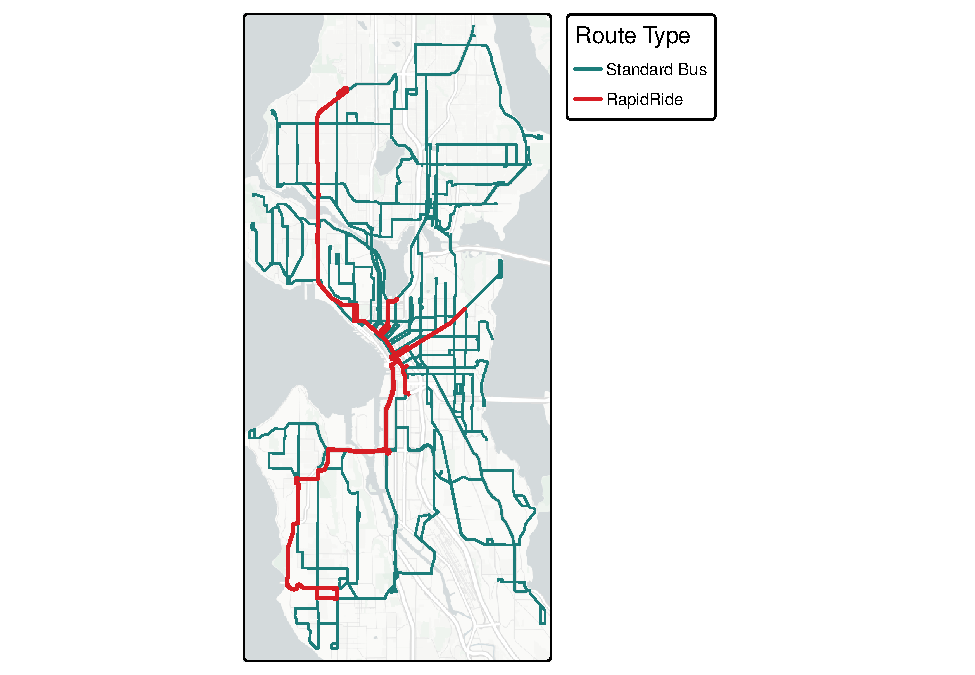
\includegraphics{thesis-draft-1_files/figure-latex/unnamed-chunk-7-1.pdf}
\caption{Map of Standard and RapidRide Bus Service in Seattle, WA.
Sources: King County Metro, CartoDB.}
\end{figure}

\subsection{2.4 The Social Implications of Transit
Performance}\label{the-social-implications-of-transit-performance}

Mass transit, in addition to being a policy needed for sustainability
goals, is a social justice policy. Given that a good, reliable transit
system increases accessibility to the city at large, equitable and
efficient dispersion of quality mass transit options allows for diverse
groups of people to access more areas of the city, opening up job and
recreation opportunities. Add to this the finding expressed previously
that individuals of lower socio-economic status are more likely to be
reliant on mass transit options. This is an issue that is particularly
pertinent in Seattle, a city with a deep history of race-based redlining
that carries forward into highly racially homogenized neighborhoods
today (Gregory, 2024). In addition, Seattle is a highly vertical
city--much longer along the North/South axis than it is wide from West
to East. Historically, poorer and less-white neighborhoods tend to be
far North and far South, far away from many of the urban centers that
contain many high-quality job opportunities and well-funded
recreation/entertainment areas (Gregory, 2024). In essence, the
improvement of transit reliability is directly tied to positive outcomes
for individuals across the income and race spectrum. It has the
potential to get people to their jobs on-time on a consistent basis,
open up more job opportunities to people living further outside the
city, and increase accessibility for people and families to quality
recreation and entertainment options.

\section{3. Data Overview}\label{data-overview}

Section 3 will outline the dataset used in this study. The dataset is
not derived from a single source. Rather, it is an amalgamation of data
from several sources, joined at either the individual or group level.
The discussion will begin with an outline of data collection for the
outcome variable, absolute deviation from schedule (AD), and then pivots
to a discussion of which pretreatment covariates were selected and the
operationalization of these variables.

\subsection{3.1 Outcome Data Overview}\label{outcome-data-overview}

The dataset started with the outcome variable, AD. Real-time bus arrival
times are reported by King County Metro via the General Transit Feed
Specification (GTFS), a standard reporting framework for transit
agencies. The real-time GTFS feed is available for public access via an
application programming interface (API). A request can be made to the
API, which will return a list of every stop in the transit network, each
of which has a series of real-time timestamps for recent arrivals at
that stop. These GTFS data are organized in a roughly hierarchical way.
The highest level of this hierarchy is the system as a whole, which can
be split into routes. Routes are the geographical multiline segments on
which trips run. Trips are unique by day, meaning only one instance of a
trip\_id is seen per day. Further, trips are directional, meaning it can
be seen via an indicator variable in the data which direction along a
route the trip travels. Along each trip are stops---pairs of (x, y)
coordinates at which busses stop to load and unload passengers. It is
important to aggregate stops under trips (rather than routes), because
directionality is important. Stop 2 going one way is the second-to-last
stop going the other way. So, each row in the dataset represents a
combination of route, trip, and stop identifiers, which are unique by
day. For the data collection in this study, requests were made to the
API on an automated schedule (every 15 minutes from 4am to 12am, local
time, between 1/29/2025 and 3/31/2025). This procedure resulted in over
4 million rows of observations, from which approximately 54,000 were
sampled for model training and test purposes. Scheduled arrival times
were appended to the dataset by trip\_id/stop\_id combination. The final
outcome variable, AD, is the absolute difference between the actual
arrival time and scheduled arrival time, in seconds. Seconds as a unit
were chosen because they represent the most granular unit of reporting
available. There was an open question as to whether the outcome variable
should discriminate between positive and negative (i.e., whether the bus
arrives early or late) or simply be absolute deviation (always
positive). The choice of AD was made because to use the
positive/negative outcome would have likely required some two-stage
modeling with a step to predict whether the arrival delay would be
positive or negative, and then a step to predict the magnitude. AD is a
simpler construct to model and a bus arriving early or late impacts the
rider in much the same way---it often means increased wait times.

\subsection{3.2 Covariate Data Overview}\label{covariate-data-overview}

Length of segment and the RapidRide indicator variables are available
via the GTFS static files provided by King County Metro. Length of
segment denotes the distance, in meters, that the bus has traveled
before any given stop. Length of segment is a directional variable and
so was joined to the main dataset by trip. The RapidRide indicator was
assigned based on route\_id. There are three RapidRide routes present in
the dataset, accounting for approximately 16 percent of the
\textasciitilde54,000 sampled observations. Traffic conditions, another
important predictor from the literature, was somewhat more difficult to
translate into the dataset. Publicly-available studies of Seattle
traffic either reported traffic levels as a function of time (e.g.,
traffic levels by hour, by day) or as a function of space (e.g., levels
of traffic on major arterials), but not both. Both were added separately
to the dataset. Though it is not necessary to standardize variables for
use in a BART, both traffic datasets were standardized for better
interpretability. Rather than trying to conceptualize how relative
vehicle volumes compare to each other, standardization provides a simple
intuition where a value of 0 means the observation has an average level
of traffic, a 1 indicates the level of traffic is 1 standard deviation
above the mean, and a -1 means the level of traffic is 1 standard
deviation below the mean. The temporal traffic dataset was available on
the Seattle Open Data Portal. Each row in this dataset represents a
study conducted on a specific date and reports the traffic volume
observed during each hour in the day. The dataset was filtered to keep
only studies conducted from 2015 onwards and excluded 2020 and 2021 due
traffic disruptions from the COVID-19 pandemic. After these operations,
there were 134,170 rows remaining in the dataset. A traffic volume
number was appended to each entry in the main dataset, corresponding to
the average traffic volume for the weekday and hour that the entry was
from. Spatial traffic data came from a 2018 study (the most recent such
study) by the Seattle Department of Transportation and contains traffic
volume for each arterial in the city. In order to join these data to the
main dataset, spatial overlays were required. King County Metro reports
the shapefiles for their bus routes, which are multiline strings. One by
one, these were overlayed on the spatial traffic geometry (also
multiline strings), which were clipped so that only the pieces of the
arterials that overlapped with the route shape remained. Then, a
weighted average of traffic volume was calculated by multiplying the
traffic volume for each arterial by the proportion of the route line it
covered. Although all bus routes had some level of coverage from the
traffic dataset, not all routes had 100\% coverage. This is due to a
lack of coverage by the traffic dataset and does represent a minor
limitation to the analysis. The next set of predictors are four
demographic variables: population density, ridership percentage,
percentage white, and median household income. Empirical studies have
shown that a high volume of ridership tends to predict decreased bus
reliability, as a function of increased boarding times, thereby
increasing dwell time. Regrettably, the real-time GTFS data used for the
outcome variable was not high-resolution enough to report on dwell times
(actual arrival and departure times were nearly always identical), so it
was necessary to operationalize dwell time in a different way. The
American Community Survey (ACS) 5-year estimates (2019-2023) reports the
estimated percentage of each census block group that uses the bus to get
to work, which gives a rough idea of the demand for busses along each
route. Because transit ridership has been shown to be positively related
to areas of lower income, higher non-white percentage, and high density,
these variables were also included to better capture variation predicted
by high ridership. Again, the route geometry was used---a quarter-mile
buffer was drawn around each route, census block groups with over 50\%
of their area within the buffer were selected, and a weighted average
ridership percentage was calculated using block group population as the
weighting variable. The quarter-mile buffer was selected because it is a
commonly used distance threshold for zoning and policy requirements
pertaining to bus lines (Puget Sound Regional Council, 2015). For
computational resource reasons, these variables were calculated at the
full route level, as opposed to the approach used for spatial traffic.
The final covariates in the dataset are weekday and hour. Weekday takes
the form of an integer with range 1-7, with 1 corresponding to Sunday.
Hour takes the form of an integer with range 1-24. For hour, a 4 denotes
the 4:00 to 4:59 time period. These variables were included as key
structural elements to the data, primarily designed to handle
commuter-based variation in the data that is likely to arise on weekdays
during peak hours.

\section{4. Methods}\label{methods}

Section 4 will review the conceptual background underpinning causal
inference and modeling techniques as they pertain to transit
reliability.

\subsection{4.1 Regression, Causal Inference, and Observational
Studies}\label{regression-causal-inference-and-observational-studies}

Causal inference is the process of creating the counterfactual. That is,
comparing potential outcomes under different applications of some
treatment or intervention (Gelman et al, 2002). In this case, the goal
is to compare potential outcomes for a route that did receive the
RapidRide upgrade ``treatment'' versus if the same route had not
received the treatment. Of course, it is impossible to simultaneously
observe a route under both treatment and no-treatment conditions.
Further, assignment of the RapidRide treatment is not random, so the
analysis cannot proceed under the assumptions that accompany a
randomized experiment. This lack of randomness is made clear in
materials produced by King County Metro---routes selected for RapidRide
upgrades are among the busiest, high-frequency routes in the city. They
tend to run along busy traffic corridors and to/through high residential
and job density zones (King County Metro, 2021). This lack of random
assignment creates further work and consideration in the analysis and
will be revisited later in this section. For now, the basic formulation
of the causal regression model is as follows:

\[Eq 1: Y \sim \beta X + \theta z + \varepsilon\]

In equation 1, Y represents the outcome (in this case, absolute
deviation from schedule, in seconds, for a given bus at a given bus
stop). X is the matrix of pretreatment covariates and \(\beta\) is the
vector of coefficients for each of these pretreatment variables.
Finally, z is the treatment indicator and is equal to 1 for routes who
have had the RapidRide treatment applied to them and 0 for routes who
have not. \(\theta\) is the coefficient on z, or the treatment effect.
Given that these data are observational, the pretreatment covariates X
are particularly important. The regression must adjust for these,
otherwise the treatment effect is prone to biases resulting from an
imbalanced sample or systematic differences across the treatment and
control groups. In this context, it is probable that average traffic
congestion, for example, is higher along RapidRide routes than among
non-RapidRide routes. The \(\beta X\) term in the regression equation
adjusts for such differences and (theoretically) gives an unbiased
estimate of the difference in outcome y between the control and
treatment groups (henceforth called the treatment effect). Indeed, it
can be shown that, in a hypothetical observational study in which there
is only one pretreatment variable that impacts both the control and
treatment groups, adjustment for this variable will return an unbiased
estimate of the treatment effect (Gelman et al, 2002). Of course, in the
real world there is not a single pretreatment variable but rather many,
and thus the adjustment procedures in the regression can only hope to do
as much adjustment as possible to reduce bias. The following section
outlines the model of choice for this study, Bayesian Additive
Regression Trees, which will be compared to a traditional multivariate
linear regression.

\subsection{4.2 Bayesian Additive Regression
Trees}\label{bayesian-additive-regression-trees}

Bayesian Additive Regression Trees (BART) is a nonparametric modeling
procedure based on ensemble machine learning methods (Chipman et al,
2010). It provides a nonparametric regression modeling approach through
decision trees, avoids overfitting (a common issue with decision trees)
through a regularization prior, gives accurate estimates of posterior
uncertainty, and elegantly handles heterogeneous treatment effects
(Hill, 2011). In a mass transit-focused paper, it is worth stating that
Bayesian Additive Regression Trees (BART) should not be confused with
Bay Area Rapid Transit (BART). There will be no further mention of Bay
Area Rapid Transit. Like many Bayesian models, BART uses the Monte Carlo
Markov Chain (MCMC) algorithm, a statistical computing algorithm that
draws samples from a probability distribution through a random walk,
iteratively fitting models. For BARTs, each chain successively builds
upon the fit of previous trees, and overfitting is reduced through the
regularization prior (Chipman et al, 2005).

\subsection{4.3 BARTs for Causal
Inference}\label{barts-for-causal-inference}

The basic regression tree is a simple machine learning model which
creates a series of partitions within the data. The tree begins with a
root node, representing a proper subset of the data. From there, the
tree performs a series of binary splits (each split is called an
interior node), creating a branching series of decision rules that
classify the data. At the bottom of the tree, the terminal nodes (also
known as leaves) represent the final subgroups and give the mean value
of the outcome for observations within these subgroups. A tree is said
to have depth 5 if there are 5 decision rules in the longest path from
the root node to a terminal node. In regression trees, the algorithm
seeks to minimize residual standard error---that is, minimize the
average difference between the value of each terminal node and the
values of the observations within those nodes (Chipman et al, 2010). In
terms of notation, T represents a binary tree consisting of some number
of internal and terminal nodes. \(M = {\mu_1, \mu_2, …, \mu_b}\)
describes the set of parameter values corresponding to each of the b
terminal nodes in the tree T. A single regression tree can be expressed
in the following way:

\[Eq 2. Y \sim g(x; T, M) + \varepsilon,\quad \varepsilon \sim N(0, \sigma^2)\]

In equation 2, the outcome Y is given by the function \(g(x; T, M)\),
which returns a predicted value for an observation with the set of
covariates x. The residual error, e, is assumed to come from a normal
distribution with mean 0 and standard deviation sigma. This is analogous
to the conditional mean of Y given x, \(E(Y | x)\) (Chipman et al,
2010). A fundamental issue with regression trees is overfitting. Left
unchecked, with no limit on depth, the tree will eventually end up with
n terminal nodes, where n is the number of observations in the sample,
thus fitting the data perfectly. To address this, BARTs use a
sum-of-trees approach combined with a regularization prior (the
``Additive'' and ``Bayesian'' parts of the BART). This approach seeks to
combine a high number of trees while minimizing the amount that each
tree contributes to the overall fit through the regularization prior
(Chipman et al, 2010). In BARTs, each tree is considered a ``weak
learner,'' meaning the algorithm limits its depth and enforces a strong
prior on each terminal node that shrinks its prediction towards 0
(Chipman et al, 2005). The BART model is the sum of many of these trees,
and can be expressed with similar notation to that of the single tree:

\[Eq. 3: Y = \sum_{j=1}^{m} g(x; T_j, M_j) + \varepsilon, \quad \varepsilon \sim N(0, \sigma^2)\]

The BART approach treats this sum of trees as the model, and uses the
Markov chain Monte Carlo (MCMC) algorithm to iteratively perturb the
weak learning trees to improve the fit (Chipman et al, 2005). These
perturbations can take the form of adding nodes to the tree (growing),
removing nodes from the tree (pruning), or altering a split rule
(changing) (Kapelner and Bleich, 2016). It is worth mentioning that the
changing perturbation is only applied to singly internal nodes---ones
where both child nodes are terminal nodes (Kapelner and Bleich, 2016). A
big relative advantage of BARTs over other ensemble regression tree
approaches (e.g., random forest, gradient boosting) is their ability to
produce coherent posterior intervals in addition to point estimates
(Hill, 2011). The algorithm samples from the posterior distribution via
MCMC to quantify uncertainty and behave well. For example, posterior
intervals are likely to be wider for predictions at test points farther
from the training data set (Chipman et al, 2005).

\subsection{4.4 Choice of Estimands and Posterior
Uncertainty}\label{choice-of-estimands-and-posterior-uncertainty}

In cases such as the present research, where multivariate models with
interaction effects and non-parametric approaches are used, regression
coefficients cannot be directly interpreted as the treatment effect.
Rather, an average treatment effect must be calculated by having the
model predict the outcome for a sample set of observations and a
counterfactual set of these observations (Gelman et al, 2002). Because
this study is focused on the effect of the RapidRide intervention, the
sample average treatment effect among the treated (SATT) chosen as the
causal estimand. Calculating the SATT involves filtering the sample to
include only observations that were treated (in this case RapidRide ==
1), and using the model to predict fitted values of AD for each
observation. Then, the treatment variable is set to the counterfactual
(RapidRide == 0) for each of the treated observations, and the model is
used to predict fitted values of AD for each of these counterfactual
observations. Finally, the counterfactual prediction is subtracted from
the factual prediction across each observation and averaged across the
sample, producing the SATT. A major strength of Bayesian approaches is
in achieving posterior uncertainty in this estimate. Both the
multivariate linear and BART models produce posterior simulation draws
(4000 draws for the multivariate linear and 2000 draws for the BART),
representing uncertainty in the parameters of the model. The procedure
above is repeated for each draw, producing a distribution in individual
treatment effects and, thus, a distribution of SATT estimates. The
standard deviation of these estimates can be examined to see to what
degree the SATT tends to be different from 0 and a confidence interval
can be constructed. In this paper, the standard 95\% confidence interval
is used, in line with most social science literature.

\section{5. Analysis and Results}\label{analysis-and-results}

Section 5 will begin with exploration and discussion of descriptive
statistics and assessments of sample balance for causal inference, and
then move to model design and evaluation, in which three models will be
outlined and tested. Finally, SATT estimates and intervals will be
calculated using both Multivariate Linear Regression and BART models.

\subsection{5.1 Descriptive Statistics}\label{descriptive-statistics}

\begin{longtable}[]{@{}
  >{\raggedright\arraybackslash}p{(\columnwidth - 14\tabcolsep) * \real{0.2794}}
  >{\raggedleft\arraybackslash}p{(\columnwidth - 14\tabcolsep) * \real{0.1029}}
  >{\raggedleft\arraybackslash}p{(\columnwidth - 14\tabcolsep) * \real{0.1176}}
  >{\raggedleft\arraybackslash}p{(\columnwidth - 14\tabcolsep) * \real{0.0882}}
  >{\raggedleft\arraybackslash}p{(\columnwidth - 14\tabcolsep) * \real{0.0882}}
  >{\raggedleft\arraybackslash}p{(\columnwidth - 14\tabcolsep) * \real{0.1029}}
  >{\raggedleft\arraybackslash}p{(\columnwidth - 14\tabcolsep) * \real{0.1029}}
  >{\raggedleft\arraybackslash}p{(\columnwidth - 14\tabcolsep) * \real{0.1176}}@{}}
\caption{Descriptive Statistics}\tabularnewline
\toprule\noalign{}
\begin{minipage}[b]{\linewidth}\raggedright
Variable
\end{minipage} & \begin{minipage}[b]{\linewidth}\raggedleft
Mean
\end{minipage} & \begin{minipage}[b]{\linewidth}\raggedleft
Std Dev
\end{minipage} & \begin{minipage}[b]{\linewidth}\raggedleft
Min
\end{minipage} & \begin{minipage}[b]{\linewidth}\raggedleft
25\%
\end{minipage} & \begin{minipage}[b]{\linewidth}\raggedleft
Median
\end{minipage} & \begin{minipage}[b]{\linewidth}\raggedleft
75\%
\end{minipage} & \begin{minipage}[b]{\linewidth}\raggedleft
Max
\end{minipage} \\
\midrule\noalign{}
\endfirsthead
\toprule\noalign{}
\begin{minipage}[b]{\linewidth}\raggedright
Variable
\end{minipage} & \begin{minipage}[b]{\linewidth}\raggedleft
Mean
\end{minipage} & \begin{minipage}[b]{\linewidth}\raggedleft
Std Dev
\end{minipage} & \begin{minipage}[b]{\linewidth}\raggedleft
Min
\end{minipage} & \begin{minipage}[b]{\linewidth}\raggedleft
25\%
\end{minipage} & \begin{minipage}[b]{\linewidth}\raggedleft
Median
\end{minipage} & \begin{minipage}[b]{\linewidth}\raggedleft
75\%
\end{minipage} & \begin{minipage}[b]{\linewidth}\raggedleft
Max
\end{minipage} \\
\midrule\noalign{}
\endhead
\bottomrule\noalign{}
\endlastfoot
RapidRide & 0.16 & 0.37 & 0.00 & 0.00 & 0.00 & 0.00 & 1.00 \\
Absolute Deviation & 210.64 & 233.62 & 0.00 & 64.00 & 147.00 & 276.25 &
3527.00 \\
Distance Traveled & 0.00 & 1.02 & -1.30 & -0.80 & -0.24 & 0.62 & 3.51 \\
Traffic (Day/Hour) & 0.00 & 1.00 & -2.74 & -0.79 & 0.25 & 0.67 & 1.52 \\
Traffic (Location) & 0.01 & 0.99 & -1.51 & -0.53 & -0.15 & 0.45 &
7.81 \\
Population Density & 0.00 & 1.01 & -1.82 & -0.56 & -0.24 & 0.65 &
2.49 \\
Route Ridership & -0.01 & 1.08 & -3.54 & -0.78 & -0.11 & 0.72 & 2.95 \\
Percentage White & 0.04 & 0.97 & -2.40 & -0.35 & 0.20 & 0.70 & 2.04 \\
Median HHI & 0.05 & 0.99 & -2.03 & -0.76 & 0.33 & 0.79 & 1.68 \\
Weekday & 3.79 & 1.93 & 1.00 & 2.00 & 4.00 & 5.00 & 7.00 \\
Hour & 14.56 & 5.08 & 1.00 & 10.00 & 15.00 & 19.00 & 24.00 \\
\end{longtable}

The exploratory data analysis process begins with an overview of the
data, variables, and their characteristics. Table 1 contains basic
descriptive statistics across the outcome, treatment, and pre-treatment
variables in the sample. RapidRide has a mean of 0.16, indicating that
the sample is comprised of 16\% of observations occurring at stops along
RapidRide routes and 85\% of observations occurring along non-RapidRide
routes. This distribution is the result of some oversampling of
RapidRide observations, as natural incidence rates of RapidRide
observations were closer to 8\%. This allows the model more information
when it comes to estimating the treatment effect but doesn't grossly
overstate the incidence of RapidRide routes in the city, which would be
the case if the sampling was done at a 50/50 level. The average AD for
observations in the sample is 210 seconds. In other words, the average
bus arrival is 3.5 minutes away from its scheduled arrival time. It is
important to note that the median observation is 147 seconds, so the
distribution is affected by some extremely late or early bus arrivals
(the greatest of which is nearly 3600 seconds, or about an hour). The
standard deviation of 233 seconds indicates very high variability for
these outcomes. The following variables were centered and standardized:
Distance Traveled, Traffic (Day/Hour), Traffic (Location), Population
Density, Route Ridership, Percentage White, and Median HHI. Each of
these variables has mean approximately equal to 0 and standard deviation
approximately equal to 1, though these are slightly changed as a result
of the RapidRide oversampling. Finally, the roughly similar values of
mean and median for Weekday and Hour indicate fairly even distributions
of observations across day and hours. For hours, though, the mean being
a bit above 12 (the presumed mean), indicates a lack of observations in
the early hours of the morning. This is expected since King County Metro
does not run buses between around midnight and 4am.

\begin{longtable}[]{@{}lrrrrr@{}}
\caption{Balance Statistics for Causal Inference}\tabularnewline
\toprule\noalign{}
& treat & control & unstd.diff & abs.std.diff & ratio \\
\midrule\noalign{}
\endfirsthead
\toprule\noalign{}
& treat & control & unstd.diff & abs.std.diff & ratio \\
\midrule\noalign{}
\endhead
\bottomrule\noalign{}
\endlastfoot
abs\_dev & 199.04 & 212.93 & -13.89 & 0.06 & 1.10 \\
shape\_dist\_traveled & 0.07 & -0.01 & 0.08 & 0.07 & 0.84 \\
avg\_traffic\_dayhour & 0.01 & 0.00 & 0.01 & 0.01 & 0.97 \\
spatial\_congestion & 0.06 & -0.01 & 0.07 & 0.08 & 1.20 \\
pop\_density & -0.04 & 0.01 & -0.05 & 0.05 & 0.96 \\
route\_ridership & -0.08 & 0.01 & -0.09 & 0.05 & 0.52 \\
perc\_white & 0.48 & -0.05 & 0.53 & 2.23 & 4.33 \\
median\_hhi & 0.60 & -0.06 & 0.66 & 0.97 & 1.46 \\
g\_weekday & 3.68 & 3.81 & -0.12 & 0.07 & 1.03 \\
g\_hr & 14.27 & 14.62 & -0.35 & 0.07 & 1.00 \\
\end{longtable}

Beyond simple descriptives, it is important to assess balance when
dealing with causal inference: do the treatment observations roughly
match the controls? Table 2 compares the raw means of the two samples in
the ``treat'' and ``control'' columns, along with the unstandardized
difference in the ``unstd.diff'' column. Further, the ``ratio'' column
provides a quick comparison---a value of 1 indicates perfect balance
between the treatment and control. The ratio for many covariates is near
1, indicating reasonable balance. There are three variables of slight
concern. Route Ridership demand is lower for RapidRide routes than for
non-RapidRide routes, and RapidRide routes tend to run though areas that
are much whiter and somewhat higher income than non-RapidRide routes.
These three variables are correlated with each other (see table 3), so
imbalance across all three of them is unsurprising. Adjustment within
the regression and BART models is designed to account somewhat for these
differences, but they do point to possible reasons that the raw
difference between the treatment and control may be misleading. Finally,
Figure 2 contains a correlation plot for each of the treatment, outcome,
and pre-treatment variables. Absolute Deviation is slightly correlated
with a number of predictors. It is worth noting that correlations
between factor variables (e.g., Weekday) are essentially meaningless and
that correlation plots do not include interaction effects, an important
piece of the models in the next section.

\begin{figure}
\centering
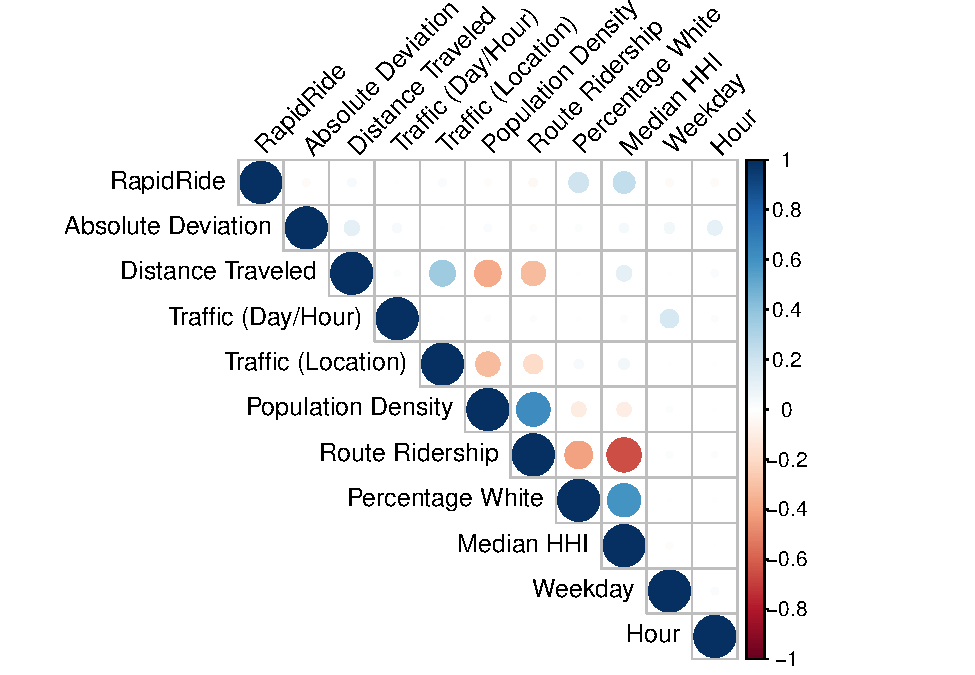
\includegraphics{thesis-draft-1_files/figure-latex/unnamed-chunk-10-1.pdf}
\caption{Correlation Plot}
\end{figure}

\subsection{5.2 Model Design and
Evaluation}\label{model-design-and-evaluation}

The present study considers three models: a simple binary linear
regression of AD on RapidRide treatment, a multivariate linear
regression of AD on RapidRide treatment and pre-treatment variables,
with interactions, and a non-parametric Bayesian Additive Regression
Trees model. Section 5.2 will give an overview of the model
specifications, assessment of model performance, and a discussion as to
which models will be used in the final analysis. The simple linear
regression of AD on the binary RapidRide treatment variable, formalized
in equation 4, produces a coefficient that may be interpreted as the
difference in means between the control and treatment groups.

\[Eq 4. AD \sim RapidRide + \varepsilon\]

As discussed earlier, though, in this observational setting it is key to
adjust for pre-treatment variables within the regression model in an
effort to account for bias and systematic differences between the
groups. Additionally, it is reasonable to think that the RapidRide
treatment may be heterogeneous for different subgroups of the data. For
example, perhaps it is more effective on certain days or hours, or in
areas of relatively higher traffic. Finally, in a simplistic effort to
capture possible nonlinearities within the data, two interaction terms
between pre-treatment variables were included: distance traveled x
traffic (day/hour) and distance traveled x traffic (location), with the
hypothesis that traffic effects get more pronounced the further the bus
has to go. As such, equation 5 formalizes the regression equation.

\[AD = \beta_0 + \beta_1 RapidRide + \beta_2 X + \beta_3 (RapidRide \times X) + \varepsilon, \quad \varepsilon \sim N(0, \sigma^2)\]

Table 4 reports the estimated coefficients for each variable, along with
standard error. Although statistical significance is not a core outcome
of interest for this study, multiplying the standard error by 2 provides
a reasonable estimate of the upper/lower bounds of a 95\% confidence
interval. First, it is clear that both models estimate a negative
relationship between RapidRide and AD, indicating that RapidRide routes
are, on average, more reliable. Further, most predictors in the
multivariate model have coefficients that are quite a bit larger than
their standard errors, meaning the model estimates they do have an
effect on the outcome. Though it is possible to go through the
interaction effects and determine the estimated effect of the RapidRide
treatment for each combination of variables, it is simpler to compute
the SATT, which will be done in the next section.

\begin{longtable}[]{@{}
  >{\raggedright\arraybackslash}p{(\columnwidth - 8\tabcolsep) * \real{0.3571}}
  >{\raggedleft\arraybackslash}p{(\columnwidth - 8\tabcolsep) * \real{0.1607}}
  >{\raggedleft\arraybackslash}p{(\columnwidth - 8\tabcolsep) * \real{0.1071}}
  >{\raggedleft\arraybackslash}p{(\columnwidth - 8\tabcolsep) * \real{0.2143}}
  >{\raggedleft\arraybackslash}p{(\columnwidth - 8\tabcolsep) * \real{0.1607}}@{}}
\caption{Linear Regression Coefficients}\tabularnewline
\toprule\noalign{}
\begin{minipage}[b]{\linewidth}\raggedright
Parameter
\end{minipage} & \begin{minipage}[b]{\linewidth}\raggedleft
Estimate (Binary)
\end{minipage} & \begin{minipage}[b]{\linewidth}\raggedleft
SE (Binary)
\end{minipage} & \begin{minipage}[b]{\linewidth}\raggedleft
Estimate (Multivariate)
\end{minipage} & \begin{minipage}[b]{\linewidth}\raggedleft
SE (Multivariate)
\end{minipage} \\
\midrule\noalign{}
\endfirsthead
\toprule\noalign{}
\begin{minipage}[b]{\linewidth}\raggedright
Parameter
\end{minipage} & \begin{minipage}[b]{\linewidth}\raggedleft
Estimate (Binary)
\end{minipage} & \begin{minipage}[b]{\linewidth}\raggedleft
SE (Binary)
\end{minipage} & \begin{minipage}[b]{\linewidth}\raggedleft
Estimate (Multivariate)
\end{minipage} & \begin{minipage}[b]{\linewidth}\raggedleft
SE (Multivariate)
\end{minipage} \\
\midrule\noalign{}
\endhead
\bottomrule\noalign{}
\endlastfoot
(Intercept) & 212.98 & 1.11 & 216.70 & 1.15 \\
rapid\_ride & -13.94 & 2.74 & -105.32 & 39.29 \\
shape\_dist\_traveled & NA & NA & 36.09 & 1.13 \\
avg\_traffic\_dayhour & NA & NA & 8.84 & 1.10 \\
spatial\_congestion & NA & NA & -6.77 & 1.16 \\
pop\_density & NA & NA & 19.08 & 1.66 \\
route\_ridership & NA & NA & -7.66 & 2.56 \\
perc\_white & NA & NA & 0.08 & 1.43 \\
median\_hhi & NA & NA & 5.46 & 1.92 \\
avg\_traffic\_dayhour:spatial\_congestion & NA & NA & 0.10 & 1.05 \\
shape\_dist\_traveled:avg\_traffic\_dayhour & NA & NA & 4.69 & 1.06 \\
shape\_dist\_traveled:spatial\_congestion & NA & NA & -11.55 & 1.21 \\
rapid\_ride:factor(g\_weekday)2 & NA & NA & 31.59 & 10.70 \\
rapid\_ride:factor(g\_weekday)3 & NA & NA & 44.80 & 11.33 \\
rapid\_ride:factor(g\_weekday)4 & NA & NA & 51.83 & 11.36 \\
rapid\_ride:factor(g\_weekday)5 & NA & NA & 41.49 & 11.88 \\
rapid\_ride:factor(g\_weekday)6 & NA & NA & 48.57 & 12.80 \\
rapid\_ride:factor(g\_weekday)7 & NA & NA & 55.07 & 11.24 \\
rapid\_ride:factor(g\_hr)4 & NA & NA & 29.19 & 84.83 \\
rapid\_ride:factor(g\_hr)5 & NA & NA & 3.48 & 46.31 \\
rapid\_ride:factor(g\_hr)6 & NA & NA & -25.96 & 35.60 \\
rapid\_ride:factor(g\_hr)7 & NA & NA & -16.51 & 35.34 \\
rapid\_ride:factor(g\_hr)8 & NA & NA & 5.18 & 37.95 \\
rapid\_ride:factor(g\_hr)9 & NA & NA & 31.98 & 39.68 \\
rapid\_ride:factor(g\_hr)10 & NA & NA & 33.74 & 38.16 \\
rapid\_ride:factor(g\_hr)11 & NA & NA & 39.44 & 37.87 \\
rapid\_ride:factor(g\_hr)12 & NA & NA & 29.30 & 37.40 \\
rapid\_ride:factor(g\_hr)13 & NA & NA & 64.96 & 38.99 \\
rapid\_ride:factor(g\_hr)14 & NA & NA & 62.70 & 38.66 \\
rapid\_ride:factor(g\_hr)15 & NA & NA & 83.67 & 40.35 \\
rapid\_ride:factor(g\_hr)16 & NA & NA & 85.16 & 40.76 \\
rapid\_ride:factor(g\_hr)17 & NA & NA & 95.47 & 42.09 \\
rapid\_ride:factor(g\_hr)18 & NA & NA & 90.48 & 41.11 \\
rapid\_ride:factor(g\_hr)19 & NA & NA & 65.12 & 40.18 \\
rapid\_ride:factor(g\_hr)20 & NA & NA & 88.39 & 37.38 \\
rapid\_ride:factor(g\_hr)21 & NA & NA & 68.81 & 35.74 \\
rapid\_ride:factor(g\_hr)22 & NA & NA & 66.97 & 36.68 \\
rapid\_ride:factor(g\_hr)23 & NA & NA & 111.42 & 35.60 \\
rapid\_ride:factor(g\_hr)24 & NA & NA & 63.80 & 37.13 \\
rapid\_ride:spatial\_congestion & NA & NA & -9.01 & 3.34 \\
rapid\_ride:route\_ridership & NA & NA & 9.70 & 2.35 \\
rapid\_ride:avg\_traffic\_dayhour & NA & NA & -19.89 & 7.85 \\
\end{longtable}

As discussed previously, one of the advantages of the BART model is its
ability to find nonlinearities within the data and look for
heterogeneous treatment effects by subgroup. The specification of the
BART model is straightforward, as can be seen in equation 6.

\[Eq. 6: AD ~ bart(RapidRide + X)\]

To compare the fit of the BART model to those of the linear regression
models, fitted predictions be compared to observed data to calculate the
Residual Mean Squared Error (RMSE), where lower RMSE indicates a better
fit. Table 6 computes and compares the RMSE for a holdout test set of
50,000 observations. Though the values are relatively similar, there is
a clear improvement between the Binary Linear and Multivariate Linear
models, as well as the Multivariate and BART models.

\begin{longtable}[]{@{}lr@{}}
\caption{RMSE by Model}\tabularnewline
\toprule\noalign{}
Model & RMSE \\
\midrule\noalign{}
\endfirsthead
\toprule\noalign{}
Model & RMSE \\
\midrule\noalign{}
\endhead
\bottomrule\noalign{}
\endlastfoot
Binary Linear & 236.36 \\
Multivariate Linear & 233.11 \\
Bayesian Additive Regression Trees & 225.40 \\
\end{longtable}

As a final aspect to the model evaluation stage, it is important to
examine the posterior residual sigma values for each chain in the BART
Model. When the model is well-specified and the algorithm is able to
converge on a parameters with relative ease, each of the four chains
mixes well with the others, producing similar values of sigma. When the
model is not well-specified, the chains often diverge and produce wildly
different values of sigma (Vehtari et al, 2021). There are two ways to
evaluate the model on this front. First, one can simply plot the values
of sigma over the iterations of each chain and visually inspect the
pattern to see if mixing has occurred. Second, one can calculate r-hat,
a metric that compares the variation in sigma within each chain to the
variation in sigma across all the chains. A value of 1 is ideal, and a
value above 1 indicates that the level of poor mixing has occurred (a
value below 1 is not possible). Standard recommendation is that a r-hat
value of less than 1.1 is ideal (Vehtari et al, 2021). Figure 3 presents
a graph of Sigma Posterior Samples by Chain, along with the estimated
r-hat of 1.18. Admittedly, this value of r-hat is above usual
recommendations, indicating that additional work should be done to
better specify the model or specify better priors. That being said, the
later estimates produced by the model are fairly coherent and time in a
master's thesis is limited, so the research proceeds with the caveat
that the model is sub-optimal.

\begin{figure}
\centering
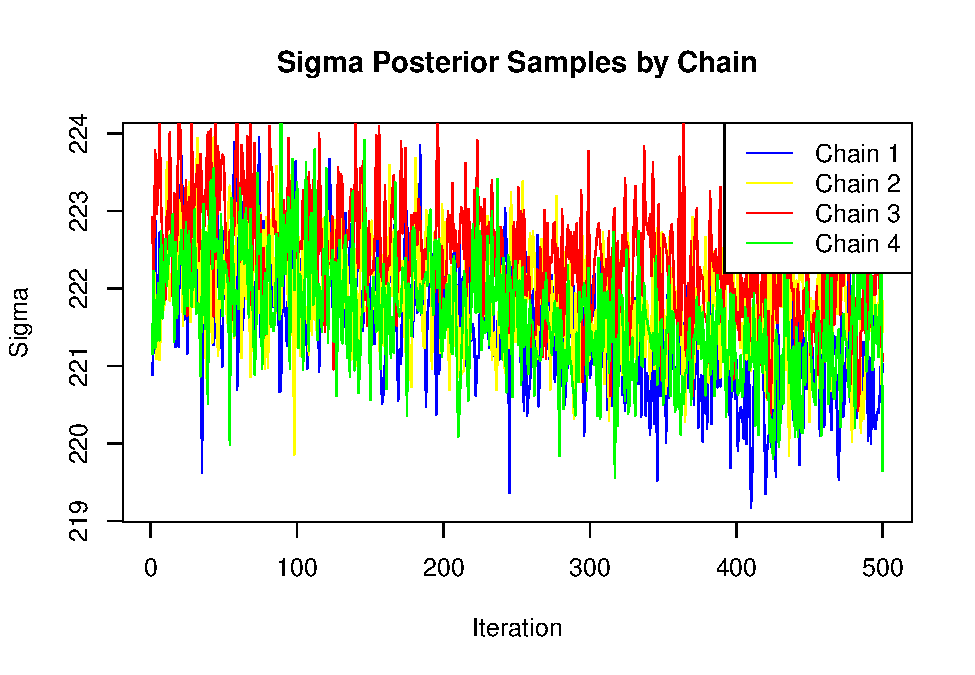
\includegraphics{thesis-draft-1_files/figure-latex/unnamed-chunk-13-1.pdf}
\caption{R-Hat = 1.18}
\end{figure}

\subsection{5.3 Causal Estimands}\label{causal-estimands}

Because of the less-than-ideal r-hat values for the BART model and the
relative similarity between the RMSE values for the BART model and
multivariate linear models, both will be used to calculate SATT
estimates. The estimates, along with their distributions, can be
examined comparatively to get a better idea of what each model is saying
about the research question and, together, they should give a decent
picture of the underlying effect.

\subsubsection{5.3.1 Sample Average Treatment Effect among the Treated
(SATT)}\label{sample-average-treatment-effect-among-the-treated-satt}

To calculate the SATT and include its uncertainty, the dataset was
filtered to only include treated observations (RapidRide == 1),
resulting in n = 8981 treated observations. Then, the dataset was copied
and all of the 1s in the RapidRide column were flipped to 0. This
provides the counterfactual---two observations that are identical across
all pretreatment variables but that differ on the treatment variable.
Each model is then used to estimate fitted predictions for each
observation. It is important to note that both models have several
thousand posterior sampling draws, so they produce several thousand
fitted values per observation. To be precise, the multivariate linear
regression produces 4000 estimates per observation and the BART model
produces 2000 estimates per observation. These estimates provide the
posterior uncertainty associated with the SATT estimates and allow for
the construction of confidence intervals. Once the predictions are made,
the counterfactual predictions are subtracted from the factual
predictions to produce individual estimates of the treatment effect for
each observation across each simulation draw. Then, the individual
estimates are averaged for each simulation draw, producing 4000
estimated SATTs for the multivariate linear model and 2000 estimated
SATTs for the BART model. These represent the estimated distribution of
the SATT. Table 5 provides the estimated median SATT for each model,
along with an upper and lower bound consistent with a 95\% confidence
interval. In this case, a negative estimate indicates a decrease in AD
and an improvement in reliability as a result of the RapidRide
treatment. Further, both models produce upper bounds that are still
negative, indicating high likelihood that the true value of the average
treatment effect among the treated is negative.

\begin{longtable}[]{@{}rrr@{}}
\caption{SATT, 95\% Confidence Interval}\tabularnewline
\toprule\noalign{}
Estimate & Lower95 & Upper95 \\
\midrule\noalign{}
\endfirsthead
\toprule\noalign{}
Estimate & Lower95 & Upper95 \\
\midrule\noalign{}
\endhead
\bottomrule\noalign{}
\endlastfoot
-48.70 & -84.05 & -11.90 \\
-15.34 & -24.04 & -6.15 \\
\end{longtable}

It is interesting, though, to examine the distributions of the estimates
of the SATT between the two models. Figure 4 present density plots of
the two distributions, with the BART distribution in blue and the
multivariate linear distribution in red. Both look normally distributed,
expected given that both models rely on the assumption of
normally-distributed error terms, but it is clear that the BART
estimates are much more variable than the multivariate linear. Given
that BARTs are designed to capture complex interactions and
nonlinearities within the data, this additional uncertainty is expected.
The more important takeaway is the relative agreement of the two models
that the effect of the RapidRide intervention is an improvement to
reliability.

\begin{figure}
\centering
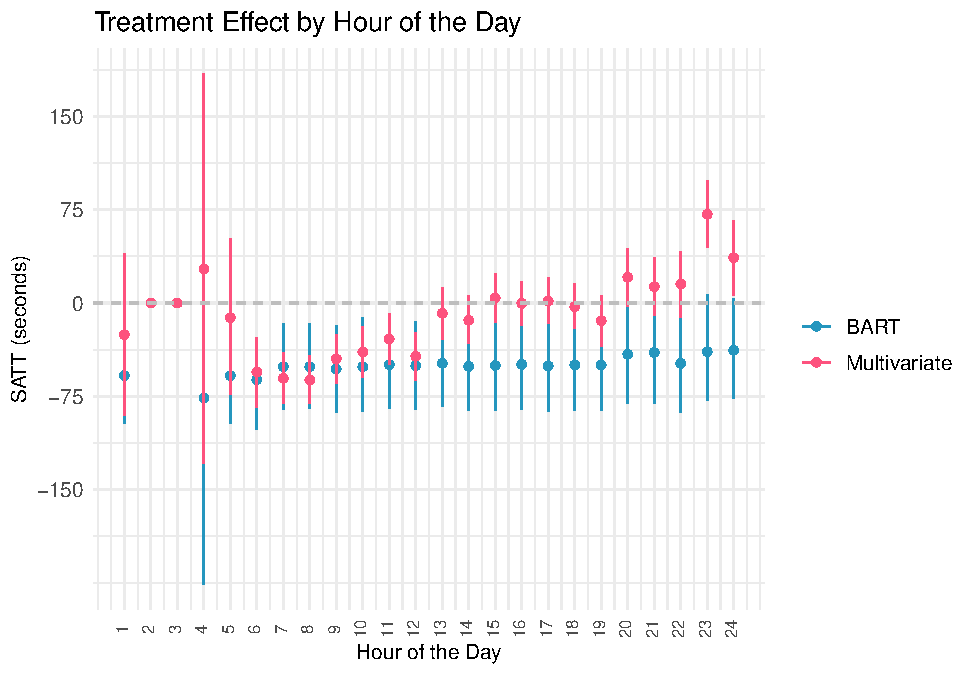
\includegraphics{thesis-draft-1_files/figure-latex/unnamed-chunk-15-1.pdf}
\caption{The distribution of SATT}
\end{figure}

\subsubsection{5.3.2 Model Comparison: Subgroup
Estimates}\label{model-comparison-subgroup-estimates}

In addition to the single estimate of SATT, it is interesting to examine
differing effects for various subgroups of the data. Not only does it
provoke interesting discussion about where and when the RapidRide
intervention is effective, but it also demonstrates further differences
between the models used. For this example, the SATT is calculated
separately for each hour of the day in the dataset. There are no
observations for hours 2 or 3, so this results in 22 distributions of
the SATT for each model. Figure 5 plots these estimates to show the
comparison between the BART and multivariate linear models. The circles
represent the median estimate, and the error bars represent a 95\%
confidence interval for the distribution. The most obvious difference
between the models is the variability of the estimates. Using the linear
regression model alone, there would be strong evidence that the
treatment effect is more pronounced between the hours of 6 and 10, and
that it disappears or even becomes negative in the afternoon and evening
hours. Conversely, the BART model shares information between subgroups,
and partially-pools the estimates, resulting in much more stable
estimates of the treatment effect. While it seems unlikely that the
treatment effect of the RapidRide intervention changes sign for the last
few hours of the day, it is not inconceivable. This is slightly
corroborated by the BART estimates---the 95\% confidence intervals for
the afternoon and evening hours often include 0. Another interesting
difference is that the confidence intervals for the multivariate linear
model are smaller than the BART for subgroups with larger samples, but
the opposite is true for hours with low amounts of observations, such as
1am and 4am. This is, again, due to partial pooling. That said, rather
than making a strict value judgement about which model is better than
the other, it is likely a better strategy to synthesize what each model
says and proceed as if both provide insights.

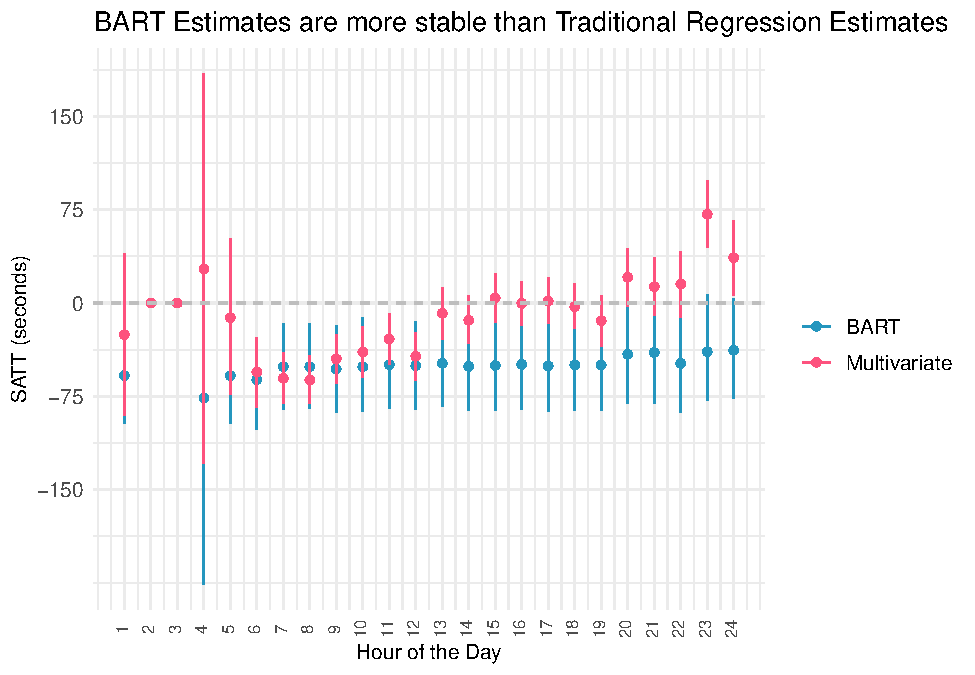
\includegraphics{thesis-draft-1_files/figure-latex/unnamed-chunk-16-1.pdf}

\section{6. Discussion}\label{discussion}

\subsection{6.1 Implication for Policy}\label{implication-for-policy}

These results are a good sign for the RapidRide system. Though it has
many stated goals, an improvement in reliability of service is a
fundamental win for the system. That being said, the magnitude of the
improvement is a question that came up time and time again through the
analysis of these results. Take, for example, the multivariate linear
results, which point to an effect of about 15 seconds. Is this worth it?
While certainly better than no change or a decrease in reliability, it
is difficult to say whether an average improvement of 15 seconds is a
worthwhile investment of several million dollars. On the other hand, the
BART estimate of almost 90 seconds seems to be a far more enticing
effect. One thing is clear---the RapidRide upgrade works when it comes
to improving reliability, so future bus routes (whether explicitly
RapidRide or not) should include these upgrades in order to continue to
propagate reliability improvements through the system. Mass transit is
an important social equity tool that should be used by the city to break
down boundaries between neighborhoods in Seattle, a city with a long
history of redlining and racial/socio-economic segregation by
neighborhood. Given that transit should be used to increase access to
the wider city from neighborhoods of a diverse range, this evidence that
the RapidRide system functions well is a signal that King County and the
City of Seattle should continue to fund the program. As was clear from
the analysis of balance between RapidRide and non-RapidRide routes, the
RapidRide routes within the city disproportionately lie in areas of
higher income and higher percentage white residents. Future routes
should focus on areas of lower wealth and higher proportions of minority
residents. Another theme that arose through the project was the idea of
granularity. In local matters especially, every dollar counts. Policy
decisions may start at the 30,000-foot, strategic priority level, but
they filter down into fundamental, small-scale decisions about
allocation of time and funding to extremely specific areas. This is a
major weakness of a lot of traditional (i.e., non-Bayesian, non-pooling)
regression methods---when the subgroups get really small, the
uncertainty gets really big. There is a common rule of thumb that you
need around 16x the sample size to effectively estimate an interaction
effect as compared to a main effect, and this rule of thumb only refers
to a single interaction, not to speak of varying treatment effects by
hour of the day, day of the week, and on a specific bus route. Through
partial-pooling and Bayesian approaches, these subgroups can at least be
estimated with a higher degree of precision, even if the smallest
subgroups are pooled in towards the overall mean. BART models are
designed to handle this sort of thing, while providing the ability to
estimate non-linearities easily, making them a really valuable tool for
causal inference moving forward.

\subsection{6.2 Limitations}\label{limitations}

Modeling is defined in large part by its limitations, and this project
is no different. Broadly, the limitations of the project can be placed
into three categories: data quality, generalizability, and model
specification. Some of the data for this project is extremely accurate.
The GTFS real-time feeds and data on route distances/RapidRide treatment
are highly accurate and suffer from essentially no missingness
whatsoever. The main data quality issue for the dataset is in the
application of covariates to individual observations. First, an ideal
dataset would include real-time traffic estimates for each observation,
rather than aggregate estimates for time and place based on historical
data. This change, simple to outline and difficult to actually
implement, would likely improve the predictive accuracy of the model by
a large margin. Additionally, the operationalization of the ridership
variable is imperfect---the census variables would be better replaced by
route-level ridership data combined with daily ridership numbers, in an
ideal world. Further, the variable set is likely insufficient to satisfy
the assumption that all confounding covariates are adjusted for within
the model. Further, the inferences associated with this study are only
truly generalizable to the time period in which the data was collected.
It may be reasonable to generalize the findings to other months and
years, but it is hard to say this without additional evidence. Lastly,
there are the previously outlined issues with model specification. The
BART model did not mix altogether well, and it is likely that the
addition of some priors or some other model specification would improve
the fit and, thus, the inference. Additionally, there are more complex
versions of the BART model that allow for concretely defined
hierarchical structure to the data (Dorie et al, 2022). These data are
structured by day and hour, as well as by stop-trip-and-route.
Accounting for these explicitly in a multilevel structure and then using
a BART term for the remaining covariates would likely provide better
causal inference than the current models.

\subsection{6.3 Future Directions}\label{future-directions}

With the limitations above addressed, this model becomes a powerful tool
for public policy researchers and decision-makers. The first future
direction for this research is a wider-scale study involving samples
from throughout a year, with further adjustment for seasonal/holiday
trends. Further, there are additional RapidRide bus routes outside of
the Seattle city limits. While all routes (RapidRide and otherwise) were
omitted from the current research because they lacked spatial traffic
data, a more inclusive study would provide better inference for the
project as a whole. A huge possibility for this research is in
cross-city comparison. Many cities have bus rapid transit systems, and
inferences across cities could be combined for a better understanding of
the intervention as a whole. The standardized GTFS structure of
real-time transit data used in cities across the US and around the world
makes data comparable across cities, which is a big boon to modeling.
Further, one weakness of the present research is that it fails to
discriminate between different aspects of the RapidRide
intervention---that is, it is unknown which part(s) of the intervention
is responsible for the positive impact on reliability. Because many
cities implement BRT differently, it may be possible to subclassify BRT
programs based on the specifics of their upgrades, and isolate which of
traffic signal priority, decreased dwell times, headway management, etc.
are most effective in improving transit reliability. Lastly, the SATT
estimates for this study were calculated on RapidRide routes, but the
procedure can be reversed, so the counterfactual turns non-RapidRide
routes into RapidRide ones. BARTs are well-suited to this task as
well---they account for uncertainty when balance and support between the
treatment and control groups are not good, meaning inference for control
observations without solid support and balance from the treatment group
would have more uncertainty associated with them. This could be used by
policymakers to identify routes with the greatest potential for
reliability improvements, alongside traditional indicators that make a
route attractive for an upgrade.

\section{7. Conclusion}\label{conclusion}

Causal inference in observational settings is hard, and the case of
RapidRide in Seattle is no different. The treatment is demonstrably
applied in a non-random way, creating a fundamental violation of the
principle of ignorability. Further, it is more interesting to examine
the current state of the program, rather than trying to achieve a
pre-post setup when the intervention was implemented, given that it
changes and evolves over time. So, the question of what effect the
RapidRide program has on the reliability of a bus route in 2025 is a
question that can only be answered with modeling and adjustment. BARTs
and multivariate linear regression both provide solutions, and the
inferences that come from these models can help inform policymakers as
to whether the intervention is successful. The present study provides an
initial result that the RapidRide intervention has the intended effect
on reliability and reduces absolute deviation from schedule on a bus
route by an average of nearly 90 seconds per minute. Further results in
subgroups provide future areas for research---granular understanding of
these patterns is paramount to better-allocated spending on mass transit
in the future.

\end{document}
